\chapter{Interpretación algebraica de la lógica}\label{sec:interp}

En este capítulo se estudiarán las principales relaciones entre la lógica proposicional y los 
polinomios con coeficientes en cuerpos finitos, centrando la atención en $\mathbb{F}_2$, 
el cuerpo finito con dos elementos.\\

La idea principal que subyace en la interpretación algebraica de la lógica es la de hacerle corresponder a cada fórmula un polinomio de forma que la función valor de verdad inducida por la fórmula se pueda entender como una función polinomial de $\mathbb{F}_2$. En otras palabras, se persigue que si la fórmula es verdadera, el valor del polinomio que tiene asociado es 1; mientras que si la fórmula es falsa, el polinomio vale 0.\\

En la Figura \ref{fig:esquema} (abajo) se muestra una representación gráfica de la relación entre las fórmulas proposicionales y los polinomios de $\mathbb{F}_2[x]$. Destacar que se usa el ideal $\mathbb{I}_2 :=(x_1+x_1^2,...,x_n+x_n^2)\subseteq\mathbb{F}_2[x]$ y que $proj$ es la proyección natural sobre el anillo cociente.

\vspace{0.5cm}
\begin{figure}[h]
	\centering
		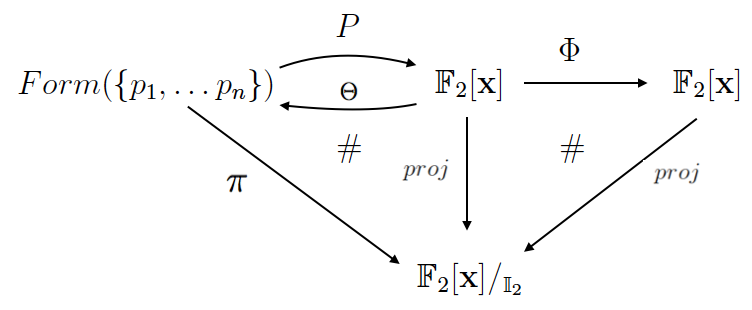
\includegraphics[scale=0.46]{imagenes/conmu.png}
	\caption{Relación entre las fórmulas proposicionales y $\mathbb{F}[x]_2$}
	\label{fig:esquema}
\end{figure}
\vspace{0.5cm}

\entrada{Logica}
\entrada{Haskell4Maths}
\entrada{F2}
\entrada{Transformaciones}